\chapter{Programação Paralela com GPU}\label{chp:LABEL_CHP_3}

Até o início dos anos 2000, o aumento na capacidade de processamento dos computadores costumava acontecer em consequência do aumento de frequência de processamento das CPUs. Esse processo foi interrompido pois não era mais possível aumentar a frequência de processamento mantendo a dissipação de calor. A forma que a indústria encontrou de manter o crescimento da capacidade de processamento dos computadores sem poder aumentar a frequência foi através da programação paralela. As CPUs passaram a ter mais de um núcleo capaz de executar diferentes instruções simultaneamente, assim, a quantidade total de processamento continuou a crescer.

O conceito de programação paralela consiste em distribuir o processamento de um programa com a finalidade de reduzir o tempo total de execução. Isso pode ser feito de algumas formas. Os programas podem executar: em diferentes núcleos de um mesmo computador, dividindo o processamento em diferentes threads ou processos; em diferentes máquinas, através de um cluster ou computação em nuvem; ou em uma CPU auxiliada por dispositivos aceleradores, como por exemplo, uma GPU, que é o foco desse trabalho.

O uso de arquiteturas diferentes em um programa não é trivial e geralmente exige um conhecimento aprofundado das capacidades de cada unidade de processamento. Por esse motivo isso não é feito de forma automática, mas sim, por meio de chamadas explícitas. Não basta encaixar uma GPU na sua placa mãe e esperar que seu programa tire proveito desse hardware, nem é possível simplesmente dizer para um programa feito para executar em CPU executar em uma GPU.
Mesmo que fosse possível, não é verdade que todo algoritmo execute melhor em um acelerador, já que eles são otimizados para casos de uso específicos.

\section{GPUs}\label{sec:GPU}
As GPUs (\emph{Graphics Processing Units}), também conhecidas como placas de vídeo, foram originalmente projetadas  como aceleradores gráficos, uma vez que seu objetivo era processar imagens rapidamente. Alguns exemplos de aplicações para GPU são: alterar a cor de todos os pixels de uma imagem, rotacionar e transladar polígonos com centenas de pontos, aplicar texturas e calcular a luminosidade nesses polígonos. 
%silvana: confusa a frase abaixo, reescrever
%Fica claro que em muitas das aplicações necessárias para uma placa de vídeo acelerar o processamento de imagens é necessário que a mesma operação seja feita em diversos pontos.
Em muitas dessas aplicações é necessário que a mesma operação seja feita em pontos distintos e independentes. Para escurecer uma imagem, por exemplo, é preciso mudar a cor de cada pixel, mas não é necessário saber a cor dos pixels em volta. 
%Como essas operações são naturalmente paralelas, as GPUs evoluíram para se aproveitar dessa característica. 
%O foco das GPUs é claramente diferente das CPUs, que tem uma ênfase muito maior em controle de fluxo e cache de dados, sua arquitetura também é diferente. 
Para se aproveitar desse paralelismo, as GPUs possuem centenas, ou até milhares de unidades lógicas, que podem executar as mesmas operações sobre blocos distintos de memória. Como podemos ver na Figura \ref{fig:gpu_1}, que modela o núcleo de uma CPU e de uma GPU, a CPU dedica muito mais espaço para controle de fluxo e cache enquanto a GPU dedica a maior parte do seu núcleo para as unidades lógicas aritméticas.

\begin{figure}
  \centering
  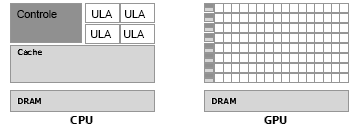
\includegraphics[width=1\textwidth]{imagens/gpu_1.png}
  \caption{As GPUs dedicam mais transistores ao processamento de dados \cite{CUDA}}
  \label{fig:gpu_1}
\end{figure}

Quando surgiram, o foco principal dessas placas era na indústria de jogos. Esse mercado bilionário impulsionou uma rápida evolução na capacidade das GPUs. Não demorou muito tempo para que os desenvolvedores vissem que as potencialidades das GPUs não estavam  limitadas à indústria de jogos. Inicialmente era muito trabalhoso usar a capacidade de processamento das placas de vídeo para aplicações de propósito geral pois era necessário conhecer APIs específicas de processamento de imagem, e saber traduzir os problemas de um domínio para o outro. Para que os desenvolvedores pudessem se aproveitar desse processamento para outros fins, os produtores de GPUs têm disponibilizado bibliotecas para executar operações de uso geral em GPUs, como o CUDA, distribuído pela NVIDIA para ser usado em suas placas gráficas.

\section{CUDA}
Lançado em 2006, CUDA \cite{CUDA} é uma plataforma de computação e um modelo de programação criado pela NVIDIA para que os desenvolvedores possam explorar o potencial das suas GPUs para aplicações de propósito geral. Atualmente, CUDA está na versão 7.5. CUDA foi desenvolvida para ser simples e facilmente compreensível por pessoas com familiaridade com linguagens de programação como C. Com CUDA é possível enviar código em C, C++ e Fortran diretamente para GPU sem precisar escrever em assembly.
%silvana: dizer de outra forma, que neste trabalho usaremos a API de CUDA para a linguagem C.
%Nesse trabalho, não estarei abordando o uso do fortran.
%Felipe: Melhor?
Neste trabalho usaremos a API de CUDA para as linguagens C e C++.
%que foram as linguagens usadas na implementação.

A base do CUDA consiste de 3 abstrações: hierarquia de threads, memória compartilhada e sincronização. Essas abstrações estão acessíveis ao programador através de comandos básicos. 

No modelo de programação de CUDA, as threads (fluxos de execução independente) são organizadas em blocos.
%A execução do CUDA em placa de vídeo é divida em blocos. Blocos são conjuntos de threads (fluxos de execução independente) 
As threads de um mesmo bloco são escalonadas para execução no mesmo núcleo de processamento e compartilham uma área de memória específica de cada núcleo. Dentro de um bloco, as threads são agrupadas em {\em warps} (conjuntos de 32 threads) para serem executadas. Cada warp é um conjunto de threads que executa perfeitamente em paralelo, ou seja, as threads executam ao mesmo tempo a mesma instrução sobre partes distintas do dado de entrada. Em caso de desvio de fluxo dentro de um warp, as threads de fluxos distintos devem aguardar o processamento das demais threads. 

O número de threads por bloco é definido pelo desenvolvedor. É recomendável que o número de threads por bloco seja múltiplo de 32, para aproveitar melhor os warps, mas a configuração que vai dar o melhor resultado, varia de aplicação para aplicação. Atualmente, nenhuma placa de vídeo suporta mais de 1024 threads por bloco, e esse valor precisa ser levado em consideração pelo desenvolvedor. Por exemplo, para executar a soma de dois vetores de 2048 elementos, seria possível configurar 2 blocos de 1024 threads com 32 warps, 4 blocos de 512 threads com 16 warps, ou 64 blocos de 32 threads em um único warp por bloco.

A escalabilidade do CUDA é feita de forma transparente para o desenvolvedor, basta fazer o programa de forma realmente paralela, onde um bloco não precise de informação de outro bloco e a ordem de execução não importe. A execução dos blocos é distribuída em tempo de execução de forma a explorar melhor a arquitetura.

\subsection{Modelo de programação de CUDA}
O núcleo do CUDA consiste de kernels, que são funções especiais compiladas para serem executadas na GPU. O kernel é definido pela declaração \texttt{\_\_global\_\_}. O número de threads e blocos que vai executar a função é especificado quando a função é chamada pela sintaxe \texttt{nomeDaFuncao< < < blocos, threads > > >(parametros...)}.
%Felipe: porque você tinha removido blocos da frase acima?

Para identificar qual thread vai processar qual dado, cada thread possui um identificador de thread, \texttt{threadIdx}, e de bloco, \texttt{blockIdx}, e é possível saber o índice do vetor que se quer acessar fazendo \texttt{indice = threadIdx.x + blockIdx.x * blockDim.x}. O \texttt{.x} serve para identificar a dimensão que estamos acessando, é possivel enviar vetores de até 3 dimensões. A quantidade de threads por bloco na dimensão {\em x} é dada pela variável \texttt{blockDim.x}.
Cada kernel tem acesso à memória privada de cada thread, à memória compartilhada por blocos de threads,  e à memória global compartilhada por todas as threads.

No Código \ref{alg:cuda_1}, apresentamos um exemplo de um kernel que eleva ao quadrado todos os elementos de um vetor. Mostramos como declarar um kernel e como usar o identificador das threads para endereçar a posição correta do vetor que cada thread deve processar.

\codec{Como escrever e invocar um Kernel}{alg:cuda_1}{codigos/cuda_1.txt}

CUDA é um modelo de programação heterogêneo onde parte do programa executa na CPU e outra parte na GPU e cada uma dessas unidades de execução possui sua área de memória.
%. Para isso, cada um executa um código distinto e possui memória distinta. 
Por isso é necessário especificar para a GPU como administrar a memória e quando executar os kernels. O CUDA oferece funções que permitem a CPU dizer para a GPU quando alocar memória, copiar dados para memória da GPU e executar os kernels.

A memória pode ser alocada na GPU através da função \texttt{cudaMalloc(\&dvcPtr, tamanho)}. É preciso salvar a referência do ponteiro da GPU pois é esse ponteiro que vai ser passado para as chamadas de kernel. Para copiar informação do \texttt{host} para o \texttt{device} (GPU), é preciso usar a função \texttt{cudaMemcpy(dvcPtr, hstPtr, tamanho,  tipo)}, onde \texttt{tipo} é um {\em enum} e pode ser \texttt{cudaMemcpyHostToDevice} ou \texttt{cudaMemcpyHostToDevice}, entre outros. Para liberar a memória alocada no \texttt{device}, usa-se \texttt{cudaFree(devicePtr)}. 

As chamadas de CUDA para o \texttt{device} pertencem à um {\em stream} que funciona como uma fila que executa os comandos na ordem que foram chamados. Algumas chamadas, como as de kernel, são por padrão assíncronas em relação ao \texttt{host}. Outras chamadas fazem a CPU eseperar a GPU terminar de trabalhar antes de continuar com o código, como \texttt{cudaMemcpy(...)} e \texttt{cudaDeviceSynchronize()}.

O programa descrito no código \ref{alg:cuda_2} utiliza muito dos conceitos que vimos. Como a alocação de memória no \texttt{device}, a cópia de um vetor do \texttt{host} para o \texttt{device}, a chamada do kernel visto em \ref{alg:cuda_1}, a cópia de um vetor do \texttt{device} para o \texttt{host} e a liberação da memória alocada na GPU.

\codec{Como alocar memória e copiar dados para GPU}{alg:cuda_2}{codigos/cuda_2.txt}

Como as funções de CUDA não executam na CPU, é difícil saber o que está acontecendo, se ocorreu um erro, ou se o programa está em um estado inválido do lado da GPU. Por isso, as funções de CUDA retornam códigos de erro ou sucesso definidos pelo {\em enum }\texttt{cudaError}. O kernel não possui esse retorno, então é necessário checar o estado da GPU após as chamadas de kernel para saber se ocorreu algum erro.  A função \texttt{cudaGetLastError()} pode ser usada para fazer essa verificação.

É possível incluir funções dentro de kernels de CUDA. Para isso é preciso colocar a diretiva \texttt{\_\_device\_\_} na assinatura da função. Dessa forma, o compilador saberá que essa função deve ser executada na GPU e para isso irá gerar o código de máquina adequado. Caso queira que a função também possa executar na CPU, é possível colocar a diretiva \texttt{\_\_host\_\_}. Assim, usando as duas diretivas é possível invocar a mesma função em códigos dentro e fora de kernels de CUDA.
